\graphicspath{{images/}}
\section{Результаты моделей}
В датасете данные можно разделить линейно, но из-за низкого количества данных точность классических алгоритмов держится в районе 80-90 процентов.

\subsection{Метод k-ближайших соседей}
\subsubsection{kNN}
\begin{alltt}
Best params: {'knn__k': 5}
Best acc: 0.9282801418439716
Accuracy: 0.9166666666666666
Recall: 1.0
Precision: 0.8648648648648649
\end{alltt}
\begin{center}
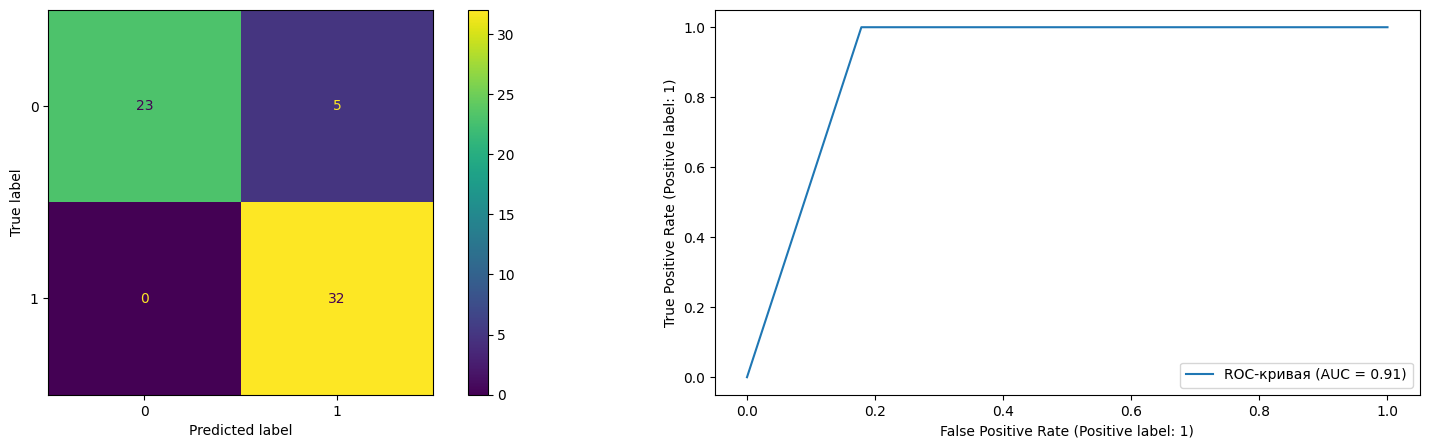
\includegraphics[width=\textwidth]{result_KNN}
\end{center}
\pagebreak

\subsubsection{sklearn.neighbors.KNeighborsClassifier}
\begin{alltt}
Best params: {'knn__n_neighbors': 5}
Best acc: 0.9282801418439716
Accuracy: 0.9166666666666666
Recall: 1.0
Precision: 0.8648648648648649
\end{alltt}
\begin{center}
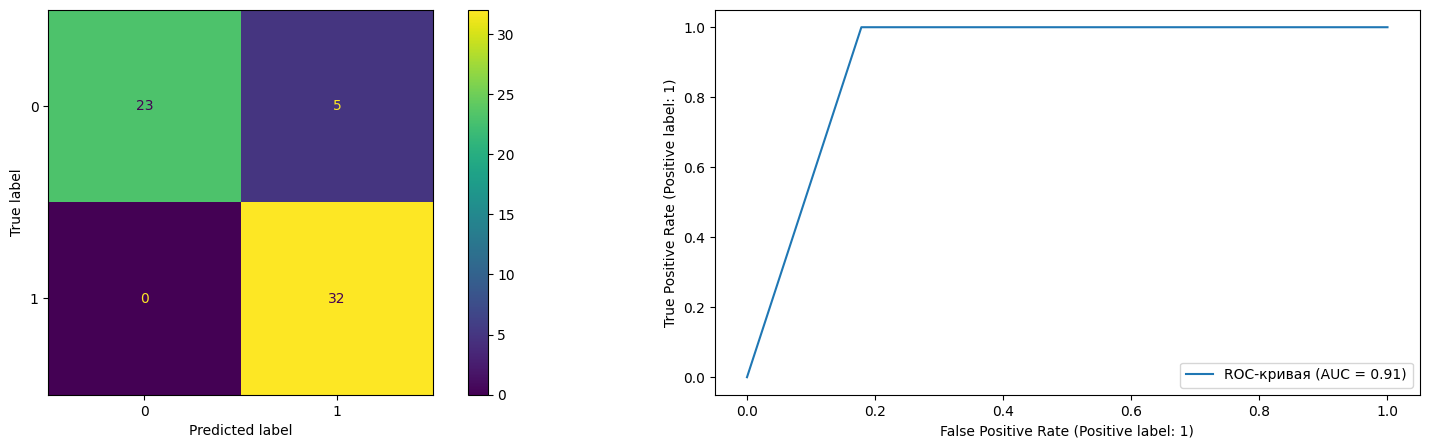
\includegraphics[width=\textwidth]{result_KNN_sc}
\end{center}
\pagebreak

\subsection{Логистическая регрессия}
\subsubsection{LogisticRegression}
\begin{alltt}
Best params: {'logreg__SGD_step': 0.01, 'logreg__batch_size': 5, 'logreg__epoches': 1}
Best acc: 0.8479609929078015
Accuracy: 0.8333333333333334
Recall: 0.78125
Precision: 0.8928571428571429
\end{alltt}
\begin{center}
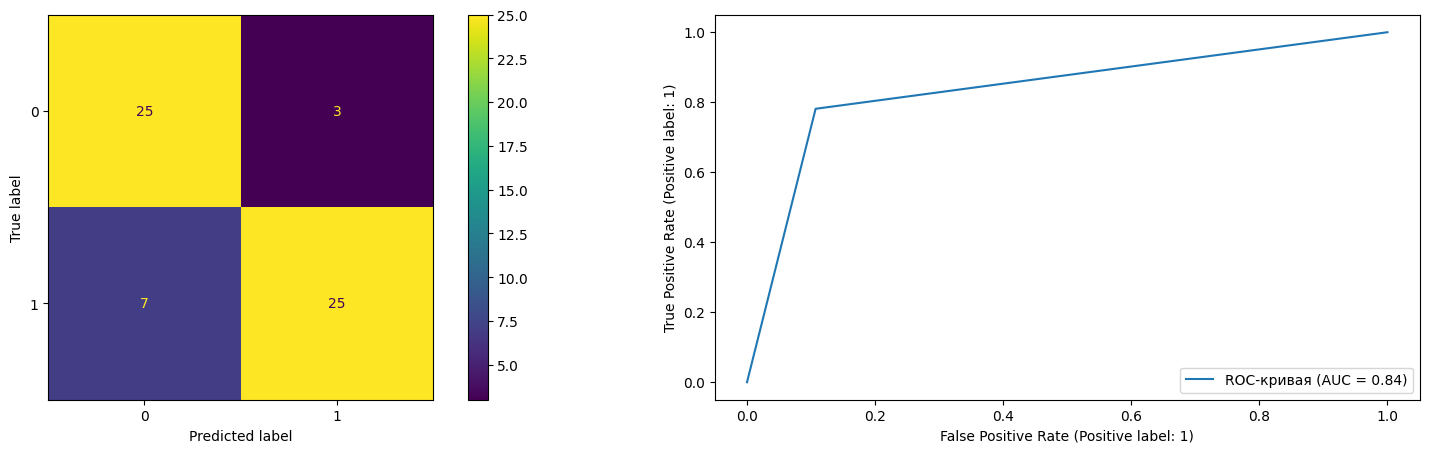
\includegraphics[width=\textwidth]{result_LR}
\end{center}

\subsubsection{sklearn.linear\_model.LogisticRegression}
\begin{alltt}
Best params: {'logreg__max_iter': 1000, 'logreg__penalty': 'l2', 'logreg__solver': 'newton-cg'}
Best acc: 0.8820035460992907
Accuracy: 0.85
Recall: 0.875
Precision: 0.8484848484848485
\end{alltt}
\begin{center}
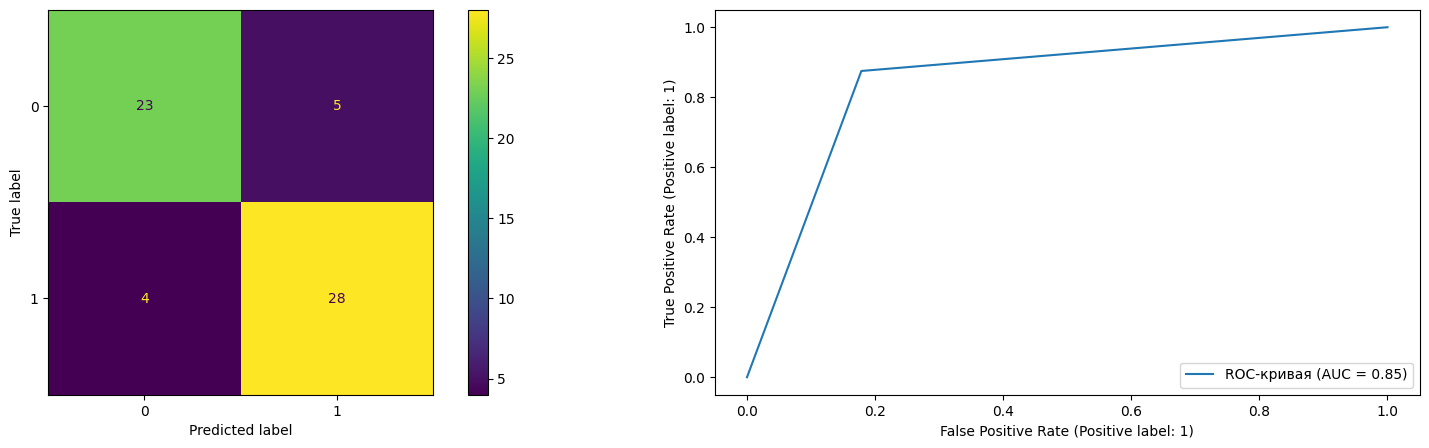
\includegraphics[width=\textwidth]{result_LR_sc}
\end{center}
\pagebreak

\subsection{Метод опорных векторов}
\subsubsection{SVM}
\begin{alltt}
Best params: {'SVM__SGD_step': 0.05, 'SVM__alpha': 0.01, 'SVM__batch_size': 20, 'SVM__epoches': 4}
Best acc: 0.8649822695035461
Accuracy: 0.8333333333333334
Recall: 0.78125
Precision: 0.8928571428571429
\end{alltt}
\begin{center}
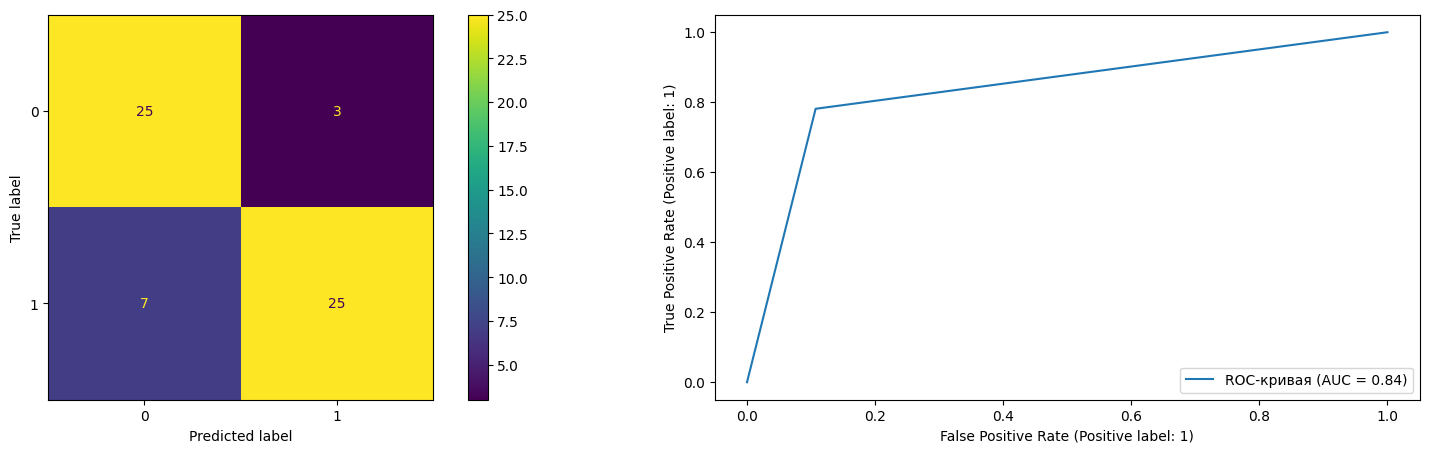
\includegraphics[width=\textwidth]{result_SVM}
\end{center}

\subsubsection{sklearn.svm.LinearSVC}
\begin{alltt}
Best params: {'svc__loss': 'hinge', 'svc__max_iter': 100000.0}
Best acc: 0.8906028368794325
Accuracy: 0.85
Recall: 0.8125
Precision: 0.896551724137931
\end{alltt}
\begin{center}
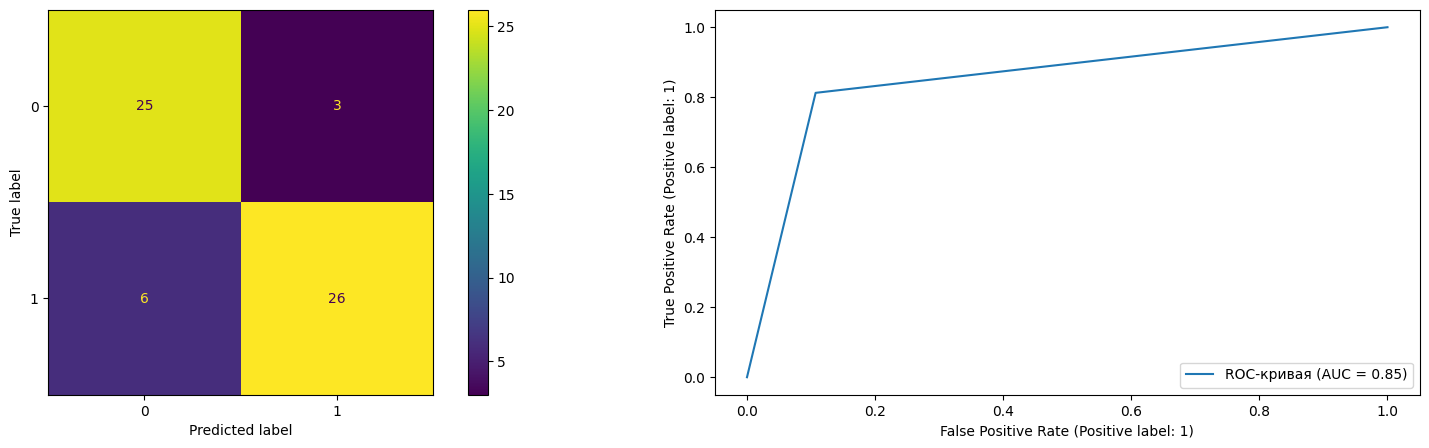
\includegraphics[width=\textwidth]{result_SVM_sc}
\end{center}
\pagebreak

\subsection{Наивный байесовский классификатор}
\subsubsection{NaiveBayes}
\begin{alltt}
Accuracy: 0.8833333333333333
Recall: 0.96875
Precision: 0.8378378378378378
\end{alltt}
\begin{center}
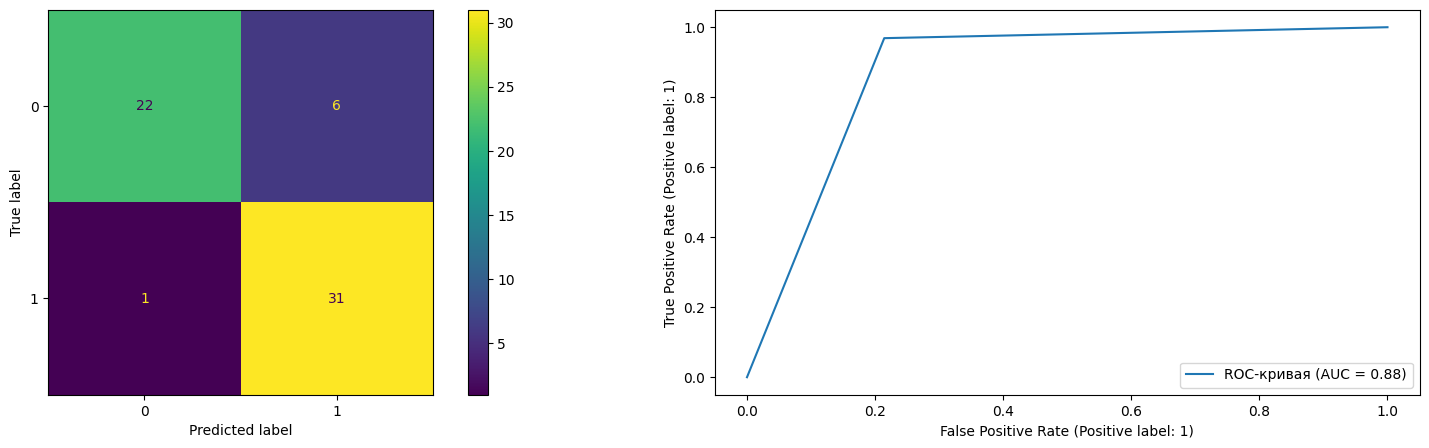
\includegraphics[width=\textwidth]{result_NB}
\end{center}

\subsubsection{sklearn.naive\_bayes.GaussianNB}
\begin{alltt}
Accuracy: 0.85
Recall: 0.84375
Precision: 0.8709677419354839
\end{alltt}
\begin{center}
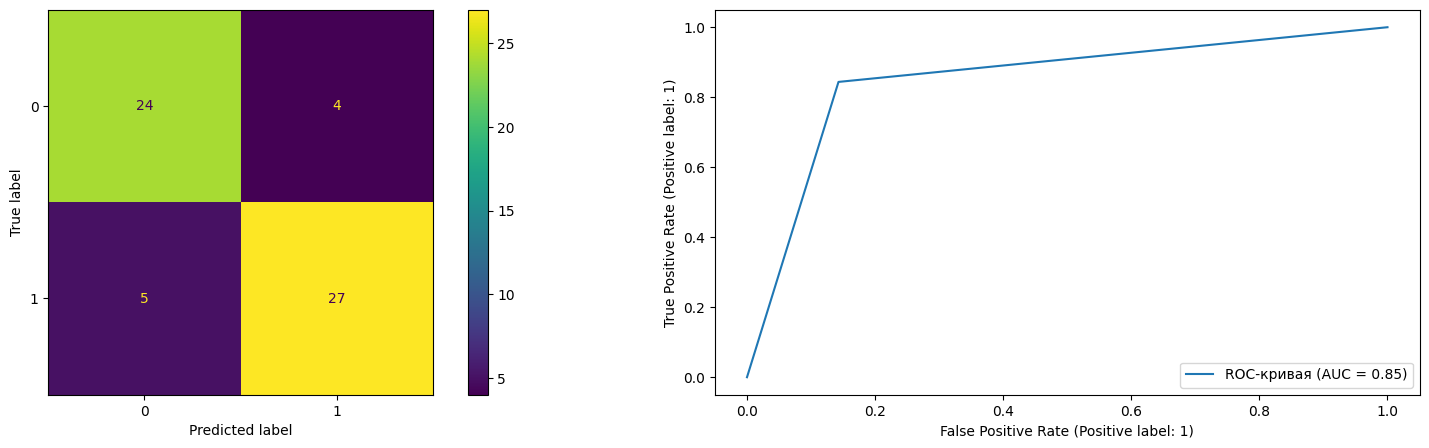
\includegraphics[width=\textwidth]{result_NB_sc}
\end{center}
\pagebreak

\subsection{Разделяющая прямая для метода опорных векторов}
\subsubsection{Моя реализация}
\begin{center}
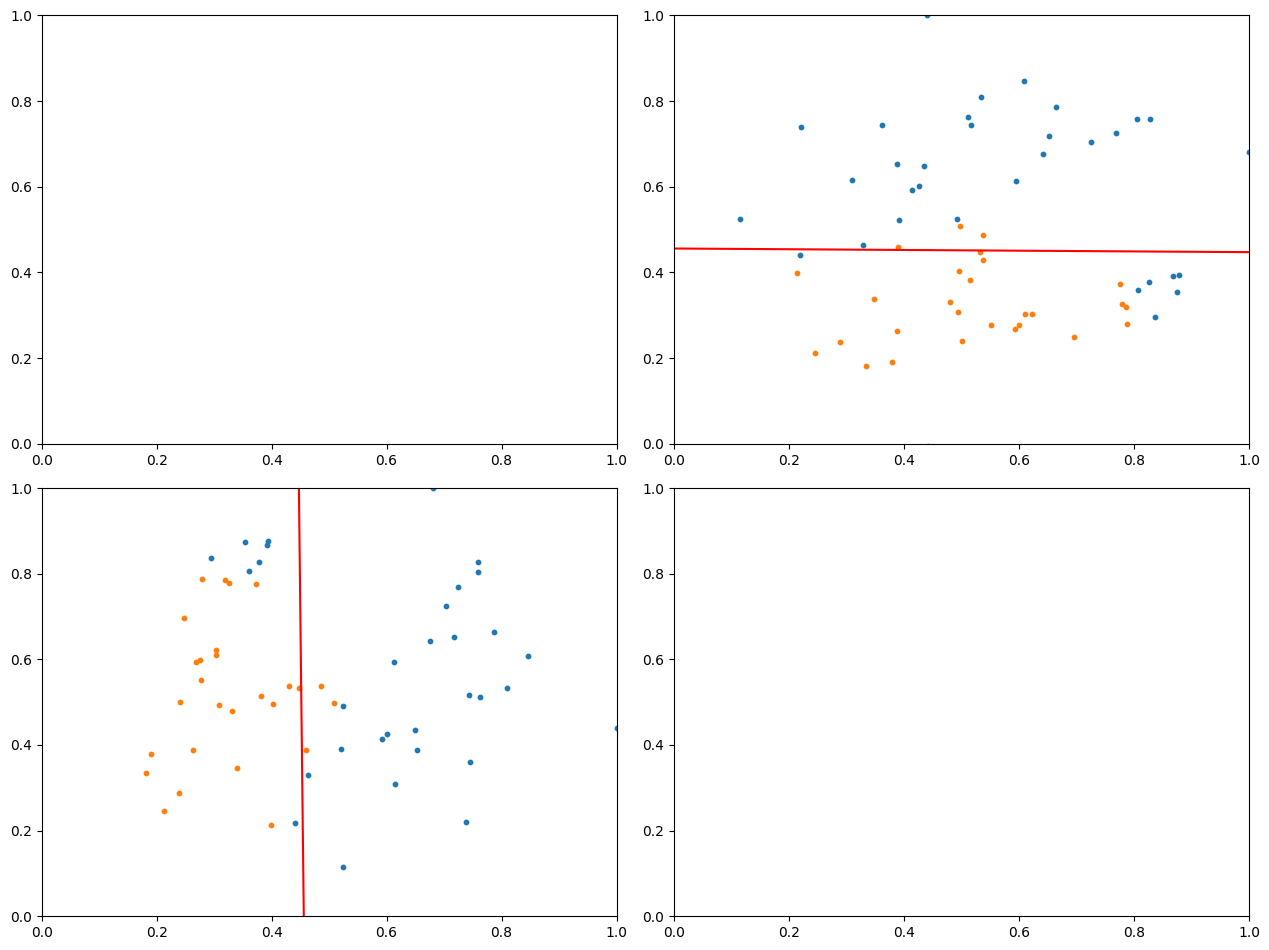
\includegraphics[width=\textwidth]{svm_lines_my}
\end{center}
\pagebreak

\subsubsection{sklearn.svm.LinearSVC}
\begin{center}
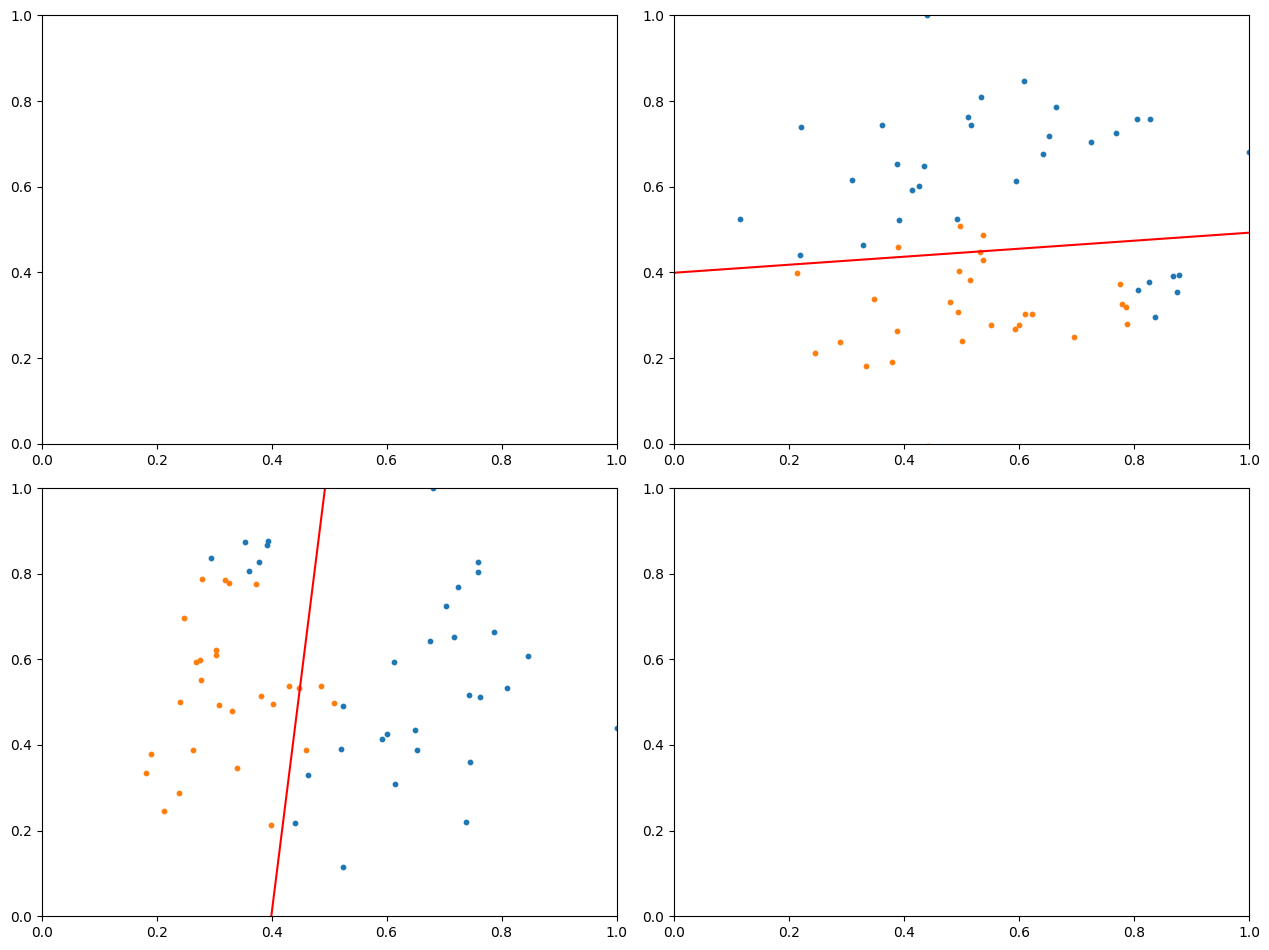
\includegraphics[width=\textwidth]{svm_lines}
\end{center}

\pagebreak
